\section{Results}

We evaluate our proposed approaches, LinkRank and LinkRank-C2I, on the ten repositories described in Table~\ref{stats}. We compare their performance against several baselines across multiple metrics.

% \noindent\textbf{\large\textit{RQ1.} How do \textsc{LinkRank} and \textsc{LinkRank-C2I} compare against existing baselines?}

\subsection{Evaluation of LinkRank and LinkRank-C2I Against Baselines}

Table~\ref{rq3} presents the average performance across ten repositories, comparing our approaches with four representative baselines: EALink, HybridLink, FRLink, and DeepLink. The results clearly demonstrate that both LinkRank and LinkRank-C2I achieve substantially higher precision, recall, and F-score than all baselines under both Known-$K$ and Unknown-$K$ regimes.


\begin{table}[htbp]
\centering
\caption{Performance (in \%) comparison of LinkRank, LinkRank-C2I, and baselines. }
\subcaption*{These values are averaged across all datasets.}
\renewcommand{\arraystretch}{1.2}
\label{rq3}
\scriptsize
\begin{tabular}{llccc}
\toprule
\multicolumn{2}{c}{\textit{\textbf{Models}}} & \textit{\textbf{Precision}} & \textit{\textbf{Recall}} & \textit{\textbf{F-score}} \\
\midrule

\multirow{3}{*}{LinkRank} 
 & Known-K     & 93.05 & 93.05 & 93.05 \\
 & No-K - ABS  & 87.04 & 92.72 & 88.80 \\
 & No-K - REL  & 83.99 & 89.92 & 85.98 \\
\midrule

\multirow{3}{*}{LinkRank - C2I} 
 & Known-K     & 92.11 & 92.11 & 92.11 \\
 & No-K - ABS  & 84.61 & 93.16 & 87.45 \\
 & No-K - REL  & 85.83 & 83.92 & 83.44 \\
\midrule

% \multirow{3}{*}{LinkRank (CodeBERT)} 
%  & Known-K     & 91.93 & 91.93 & 91.93 \\
%  & No-K - ABS  & 86.75 & 93.48 & 88.95 \\
%  & No-K - REL  & 86.52 & 82.26 & 82.78 \\
% \midrule

% \multirow{3}{*}{LinkRank - C2I (CodeBERT)} 
%  & Known-K     & 92.14 & 92.14 & 92.14 \\
%  & No-K - ABS  & 85.86 & 92.65 & 88.04 \\
%  & No-K - REL  & 85.38 & 84.39 & 83.38 \\
% \midrule

\multirow{4}{*}{Baseline} 
 & EALINK\cite{ealink}     & 57.67 & 71.73 & 61.47 \\
 & HybridLink\cite{q2}  & 61.70 & 61.70 & 58.90 \\
 & FRLink\cite{r56}      & 46.43 & 73.85 & 55.84 \\
 & DeepLink\cite{q1}   & 49.58 & 51.422 & 48.51 \\
\bottomrule
\end{tabular}
\end{table}

Under the oracle \textit{Known-$K$} setting, LinkRank achieves an F-score of 93.05\%, closely followed by LinkRank-C2I at 92.11\%. These values are substantially higher than the best-performing baseline, EALink, which records only 61.47\%. In the more realistic \textit{Unknown-$K$} scenarios, our approaches continue to perform strongly. With ABS thresholding, LinkRank attains an F-score of 88.80\% and LinkRank-C2I achieves 87.45\%, while the baselines remain in the 48\%--61\% range. Under REL thresholding, LinkRank records 85.98\% and LinkRank-C2I achieves 83.44, again well above all baselines.\\

\textbf{Takeaway:} Across evaluation regimes, both LinkRank and LinkRank-C2I consistently outperform prior baselines by large margins, often exceeding them by 25--35 points in F-score. These results demonstrate that our learning-to-rank formulation is robust, generalizable, and establishes a new state of the art for one-to-many issue--commit link recovery. The weaker performance of baseline models can be attributed to their design: as discussed in the related work, existing approaches were primarily developed for one-to-one linking and treat the problem as a binary classification task, making them not well adapted to capture the complexity of one-to-many relations.



% Under the oracle \textbf{Known-$K$} setting, LinkRank reaches an average F-score of 91.91, while LinkRank-C2I attains 87.90. These scores are markedly higher than the best baseline, EALink, which achieves only 61.47 F-score. More importantly, in the more realistic \textbf{Unknown-$K$} scenarios, our models continue to dominate. For instance, under ABS thresholding, LinkRank achieves an average F-score of 86.82 and LinkRank-C2I achieves 84.24, compared to baseline values that remain in the 48--61 range. Under REL thresholding, LinkRank-C2I achieves an average F-score of 91.42, highlighting that bidirectional refinement can be highly effective in practice.

% \textbf{Takeaway.} Averaged across ten diverse repositories, both LinkRank and LinkRank-C2I deliver large, consistent gains over prior baselines, often exceeding them by 25--35 points in F-score. This establishes that our learning-to-rank formulation is not only robust and generalizable but also sets a new performance bar for one-to-many issue--commit link recovery.



% \textit{RQ2: How effective are LinkRank and its variant  LinkRank-C2I in recovering one-to-many issue--commit links?}

\subsection{Effectiveness of LinkRank and LinkRank-C2I for One-to-Many Recovery}

Table~\ref{rq2} reports results for both approaches under three selection regimes. As expected, \textit{Known-$K$} yields high scores across datasets, but it assumes oracle knowledge of the true number of commits per issue and is therefore not a realistic deployment setting. We thus focus our analysis on the \textit{Unknown-$K$} strategies (ABS and REL), which reflect practical use.\\

\begin{table*}[htbp]
\centering
\caption{Performance (in \%) of LinkRank and LinkRank-C2I} 
\subcaption*{Across 10 datasets under three regimes: Known-K, and Unknown-K with ABS and REL.}
\renewcommand{\arraystretch}{1.3}
\label{rq2}
\begin{tabular}{@{}llcccccc@{}}
\toprule
\multirow{2}{*}{\textbf{Dataset}} & \multirow{2}{*}{\textbf{Variations}} & \multicolumn{3}{c}{\textbf{LinkRank}} & \multicolumn{3}{c}{\textbf{LinkRank-C2I}} \\
\cmidrule(lr){3-5} \cmidrule(lr){6-8}
 &  & \textbf{Precision} & \textbf{Recall} & \textbf{F-score} & \textbf{Precision} & \textbf{Recall} & \textbf{F-score} \\
\midrule

\multirow{3}{*}{Apache/Beam}
 & Known K         & 91.29 & 91.29 & 91.29 & 90.35 & 90.32 & 90.33 \\
 & Unknown-K (ABS) & 84.67 & 89.92 & 86.04 & 83.24 & 90.63 & 85.59 \\
 & Unknown-K (REL) & 78.15 & 86.69 & 81.10 & 81.59 & 79.11 & 78.58 \\
\midrule

\multirow{3}{*}{Apache/Datafusion}
 & Known K         & 93.01 & 93.01 & 93.01 & 91.06 & 91.06 & 91.06 \\
 & Unknown-K (ABS) & 84.38 & 93.22 & 87.46 & 83.99 & 92.52 & 86.86 \\
 & Unknown-K (REL) & 82.16 & 88.72 & 84.09 & 83.50 & 81.52 & 80.89 \\
\midrule

\multirow{3}{*}{Apache/Superset}
 & Known K         & 95.04 & 95.04 & 95.04 & 91.89 & 91.89 & 91.89 \\
 & Unknown-K (ABS) & 90.57 & 93.67 & 91.35 & 82.52 & 91.65 & 85.28 \\
 & Unknown-K (REL) & 87.04 & 90.26 & 87.92 & 86.71 & 83.34 & 83.82 \\
\midrule

\multirow{3}{*}{Apache/Mxnet}
 & Known K         & 92.01 & 92.01 & 92.01 & 94.31 & 94.31 & 94.31 \\
 & Unknown-K (ABS) & 86.79 & 92.79 & 89.14 & 86.43 & 94.10 & 88.98 \\
 & Unknown-K (REL) & 85.93 & 88.73 & 86.63 & 89.45 & 88.38 & 88.08 \\
\midrule

\multirow{3}{*}{Apache/Dubbo}
 & Known K         & 92.72 & 92.72 & 92.72 & 91.42 & 91.42 & 91.42 \\
 & Unknown-K (ABS) & 87.31 & 93.15 & 89.23 & 76.00 & 95.42 & 83.54 \\
 & Unknown-K (REL) & 83.17 & 91.09 & 86.11 & 85.90 & 88.18 & 85.79 \\
\midrule

\multirow{3}{*}{Apache/Iceberg}
 & Known K         & 94.22 & 94.22 & 94.22 & 94.56 & 94.56 & 94.56 \\
 & Unknown-K (ABS) & 86.81 & 94.02 & 89.52 & 91.96 & 93.55 & 91.97 \\
 & Unknown-K (REL) & 87.93 & 91.41 & 89.22 & 88.07 & 85.04 & 85.40 \\
\midrule

\multirow{3}{*}{Kubernetes}
 & Known K         & 89.03 & 89.03 & 89.03 & 93.66 & 93.66 & 93.66 \\
 & Unknown-K (ABS) & 81.92 & 87.13 & 82.83 & 87.65 & 95.92 & 90.64 \\
 & Unknown-K (REL) & 73.57 & 83.12 & 76.73 & 89.54 & 88.32 & 87.68 \\
\midrule

\multirow{3}{*}{grpc}
 & Known K         & 95.75 & 95.75 & 95.75 & 86.44 & 86.44 & 86.44 \\
 & Unknown-K (ABS) & 89.24 & 93.47 & 90.23 & 83.68 & 84.99 & 82.57 \\
 & Unknown-K (REL) & 87.06 & 94.46 & 89.74 & 78.19 & 72.00 & 72.68 \\
\midrule

\multirow{3}{*}{Tensorflow}
 & Known K         & 95.75 & 95.75 & 95.75 & 92.70 & 92.70 & 92.70 \\
 & Unknown-K (ABS) & 89.84 & 93.75 & 90.85 & 83.36 & 96.86 & 88.59 \\
 & Unknown-K (REL) & 87.95 & 92.59 & 89.40 & 86.07 & 88.31 & 85.91 \\
\midrule

\multirow{3}{*}{Pytorch}
 & Known K         & 91.70 & 91.70 & 91.70 & 94.73 & 94.73 & 94.73 \\
 & Unknown-K (ABS) & 88.89 & 96.04 & 91.39 & 87.25 & 96.01 & 90.48 \\
 & Unknown-K (REL) & 86.90 & 92.13 & 88.89 & 89.25 & 85.00 & 85.59 \\
\bottomrule
\end{tabular}
\end{table*}


Under \textbf {Unknown-$K$ (ABS)}, LinkRank achieves strong and stable performance across most repositories (e.g., Apache/Superset: F1 = 91.35\%; TensorFlow: 90.85\%; PyTorch: 91.39\%). LinkRank-C2I remains competitive and in some cases surpasses LinkRank (e.g., Apache/Mxnet: 88.98\%; Apache/Dubbo: 83.54\%; Kubernetes: 90.64\%). These results indicate that a global threshold can work well when per-issue score calibration is consistent, with the commit$\rightarrow$issue shortlist occasionally providing additional gains.\\

Under \textbf {Unknown-$K$ (REL)}, LinkRank-C2I generally outperforms LinkRank across repositories. Notable F1 scores include Kubernetes: 87.68\%, Apache/Mxnet: 88.08\%, Apache/Dubbo: 85.79\%, and PyTorch: 85.59\%, with LinkRank-C2I also remaining competitive on others (e.g., Apache/Superset: 83.82\% vs.\ 87.92\% for LinkRank, Apache/Iceberg: 85.40\% vs.\ 89.22\% for LinkRank). This suggests that relative, per-issue thresholding benefits from the bidirectional pipeline, where commit-side shortlist gating helps adapt thresholds more effectively to local project characteristics.\\


\textbf{Takeaways:}
\begin{enumerate}
    \item \textbf{Known-$K$}: serves as a useful \textbf{upper-bound diagnostic} — it quantifies the \textbf{best-case ranking quality} when the true number of commits per issue is available. However, it is an \textbf{oracle} setting and therefore not practical for deployment.
        \item \textbf{Unknown-$K$ (overall)}: both \textbf{ABS} and \textbf{REL} produce strong one-to-many recovery across diverse repositories, but they differ in behavior and assumptions:
            \begin{enumerate}
                \item \textbf{ABS (global absolute threshold)}: yields \textbf{stable, predictable performance} when model scores are consistently calibrated across issues and projects. It is simple to tune on a development set and is computationally cheap at inference.
                \item \textbf{REL (per-issue relative threshold)}: adapts to \textbf{per-issue score distributions} and better handles heterogeneity (varying numbers of true commits, sparse or noisy issue text). It often improves \textbf{recall} for issues with many relevant commits at the cost of slightly more variance.
            \end{enumerate}
        \item \textbf{LinkRank vs LinkRank-C2I}: \textbf{LinkRank} provides \textbf{robust, high F1} under \textbf{ABS}; \textbf{LinkRank-C2I} typically shines under \textbf{REL} where the \textbf{commit$\rightarrow$issue shortlist} and \textbf{bidirectional refinement} help adapt thresholds and recover more complex one-to-many relations.
\end{enumerate}
LinkRank delivers stable, high performance under ABS, while LinkRank-C2I provides a complementary, bidirectional view 
that often improves results, particularly under REL, without degrading overall robustness. 
Together, the two formulations validate that a learning-to-rank approach is well suited to issue$\rightarrow$commit set prediction, offering reliable accuracy across diverse projects and evaluation regimes.

\begin{table*}[htbp]
\centering
\caption{Performance (in \%) of LinkRank and LinkRank-C2I with CodeBERT embeddings}
\subcaption*{Across 10 datasets under three regimes: Known-K, and Unknown-K with ABS and REL.}
\renewcommand{\arraystretch}{1.3}
\label{rq1}
\begin{tabular}{@{}llcccccc@{}}
\toprule
\multirow{2}{*}{\textbf{Dataset}} & \multirow{2}{*}{\textbf{Variations}} & \multicolumn{3}{c}{\textbf{LinkRank}} & \multicolumn{3}{c}{\textbf{LinkRank-C2I}} \\
\cmidrule(lr){3-5} \cmidrule(lr){6-8}
 &  & \textbf{Precision} & \textbf{Recall} & \textbf{F-score} & \textbf{Precision} & \textbf{Recall} & \textbf{F-score} \\
\midrule

\multirow{3}{*}{Apache/Beam}
 & Known K           & 89.03 & 89.03 & 89.03 & 89.48 & 89.46 & 89.47 \\
 & Unknown-K (ABS)   & 82.73 & 91.58 & 85.53 & 84.22 & 88.91 & 85.14 \\
 & Unknown-K (REL)   & 80.84 & 76.39 & 76.57 & 80.29 & 76.94 & 76.66 \\
\midrule

\multirow{3}{*}{Apache/Datafusion}
 & Known K           & 91.45 & 91.45 & 91.45 & 90.65 & 90.65 & 90.65 \\
 & Unknown-K (ABS)   & 84.35 & 93.37 & 87.69 & 84.78 & 92.32 & 87.43 \\
 & Unknown-K (REL)   & 85.72 & 79.46 & 80.62 & 84.86 & 80.14 & 80.49 \\
\midrule

\multirow{3}{*}{Apache/Superset}
 & Known K           & 94.48 & 94.48 & 94.48 & 93.29 & 93.29 & 93.29 \\
 & Unknown-K (ABS)   & 90.64 & 94.51 & 91.79 & 88.65 & 92.28 & 89.49 \\
 & Unknown-K (REL)   & 89.31 & 85.88 & 86.60 & 87.25 & 86.50 & 86.07 \\
\midrule

\multirow{3}{*}{Apache/Mxnet}
 & Known K           & 90.94 & 90.94 & 90.94 & 94.58 & 94.58 & 94.58 \\
 & Unknown-K (ABS)   & 87.26 & 92.57 & 89.19 & 86.33 & 93.59 & 88.70 \\
 & Unknown-K (REL)   & 85.76 & 83.55 & 83.46 & 87.98 & 87.34 & 86.49 \\
\midrule

\multirow{3}{*}{Apache/Dubbo}
 & Known K           & 93.10 & 93.10 & 93.10 & 90.59 & 90.59 & 90.59 \\
 & Unknown-K (ABS)   & 88.46 & 91.81 & 89.11 & 82.48 & 91.28 & 85.57 \\
 & Unknown-K (REL)   & 87.31 & 82.64 & 83.59 & 84.12 & 87.22 & 84.53 \\
\midrule

\multirow{3}{*}{Apache/iceberg}
 & Known K           & 93.16 & 93.16 & 93.16 & 94.61 & 94.61 & 94.61 \\
 & Unknown-K (ABS)   & 88.77 & 93.51 & 90.08 & 90.06 & 94.66 & 91.61 \\
 & Unknown-K (REL)   & 87.99 & 85.53 & 85.59 & 87.35 & 85.57 & 85.41 \\
\midrule

\multirow{3}{*}{Kubernetes}
 & Known K           & 87.80 & 87.80 & 87.80 & 93.36 & 93.36 & 93.36 \\
 & Unknown-K (ABS)   & 81.46 & 91.46 & 84.93 & 88.38 & 94.63 & 90.32 \\
 & Unknown-K (REL)   & 81.78 & 70.22 & 72.97 & 88.35 & 88.15 & 86.67 \\
\midrule

\multirow{3}{*}{grpc}
 & Known K           & 94.49 & 94.49 & 94.49 & 88.02 & 88.02 & 88.02 \\
 & Unknown-K (ABS)   & 88.38 & 95.40 & 90.71 & 81.30 & 88.62 & 83.29 \\
 & Unknown-K (REL)   & 90.12 & 87.45 & 87.30 & 78.51 & 77.16 & 75.50 \\
\midrule

\multirow{3}{*}{Tensorflow}
 & Known K           & 94.62 & 94.62 & 94.62 & 92.06 & 92.06 & 92.06 \\
 & Unknown-K (ABS)   & 87.94 & 95.70 & 90.61 & 82.51 & 95.07 & 87.27 \\
 & Unknown-K (REL)   & 89.78 & 82.09 & 84.00 & 84.41 & 88.15 & 85.03 \\
\midrule

\multirow{3}{*}{Pytorch}
 & Known K           & 90.19 & 90.19 & 90.19 & 94.78 & 94.78 & 94.78 \\
 & Unknown-K (ABS)   & 87.52 & 94.85 & 89.89 & 89.89 & 95.17 & 91.62 \\
 & Unknown-K (REL)   & 86.55 & 89.36 & 87.09 & 90.63 & 86.75 & 87.00 \\
\bottomrule
\end{tabular}
\end{table*}

% \textit{RQ3: Does integrating CodeBERT embeddings improve the performance of our models?}
\newpage
\subsection{Impact of CodeBERT Embeddings on LinkRank and LinkRank-C2I}

Table~\ref{rq1} reports the results of both LinkRank and LinkRank-C2I when augmented with CodeBERT embeddings. Overall, we do not observe consistent or substantial improvements compared to the non-embedding setup: the observed gains are small, mixed across datasets, and often fall within the range of typical variance. This suggests that the core formulation of our framework already captures most of the discriminative signal required for one-to-many issue--commit recovery.

\paragraph{Why are gains limited?}
First, our learning-to-rank approach trains and evaluates \emph{per issue}, focusing on the relative ordering of candidates within each pool. Using a LambdaMART objective, the model learns complex feature interactions while emphasizing rank quality rather than absolute similarity, reducing its dependency on additional semantic channels. Second, the \emph{iterative pick--remove--renormalize} strategy with \emph{Unknown-$K$} stopping (ABS/REL) continuously recalibrates per-issue scores, further diminishing the marginal utility of transformer-based embeddings. Third, one-to-many issue--commit recovery is inherently a \emph{pattern-matching task}, where lexical embeddings naturally align issue and commit text. In this setting, the combination of TF--IDF and LambdaMART proves especially effective, leaving limited headroom for heavy semantic embeddings.

% in our PR-aware datasets, linked commits are often lexically close to their issues, enabling traditional IR-style features (e.g., TF--IDF) to perform strongly. Finally,

\paragraph{When can CodeBERT help?}
Despite limited overall gains, CodeBERT may offer benefits in cases where issue and commit descriptions are sparse, noisy, or paraphrased, or in contexts requiring richer semantic explanations or graph-structured reasoning. In such scenarios, semantic embeddings could complement lexical matching, but for the majority of real-world repositories, lightweight IR features combined with LambdaMART remain both effective and efficient.

\paragraph{Takeaway:}
Incorporating CodeBERT is optional: while it may yield modest improvements in special cases, our results show that the proposed framework already achieves strong performance without relying on computationally expensive transformer-based embeddings.





% \textit{RQ4: How do LinkRank and LinkRank-C2I perform in cross-project settings, where models trained on one programming language or repository are evaluated on others?}

\subsection{Cross-Repository Performance}

In the cross-repository experiments, we train LinkRank and LinkRank-C2I on repositories of a single programming language (Java, Go \& Rust, or C++) or a subgroup of related repositories and evaluate them on all other repositories, spanning different languages and domains. This setup tests the models' ability to generalize across diverse coding styles, terminologies, and project conventions.

% =======================
%   TRAINED ON JAVA
% =======================
\begin{figure}[H]
  \centering
  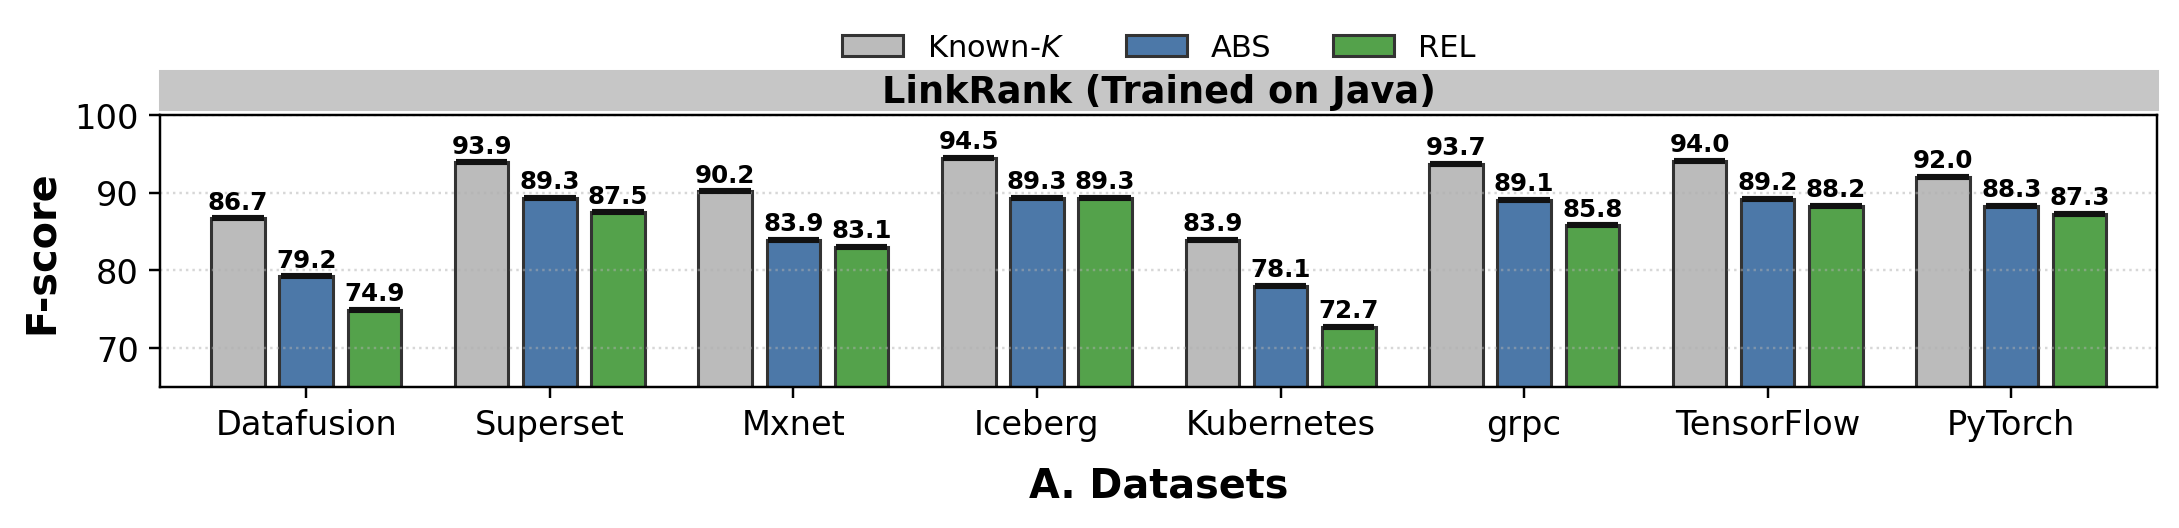
\includegraphics[width=\linewidth]{Figures/LR-java.png}
  \caption{Cross-project performance of \textsc{LinkRank} trained on Java repositories. }
  \subcaption*{Panels show per-dataset F\textsubscript{1} under Known-$K$, ABS, and REL regimes.}
  \label{fig:LR-java}
\end{figure}

\begin{figure}[H]
  \centering
  \includegraphics[width=\linewidth]{Figures/lr-C2I-java.png}
  \caption{Cross-project performance of \textsc{LinkRank-C2I} trained on Java repositories.}
  \label{fig:LR-C2I-java}
\end{figure}


% =======================
%   TRAINED ON RUST & GO
% =======================
\begin{figure}[H]
  \centering
  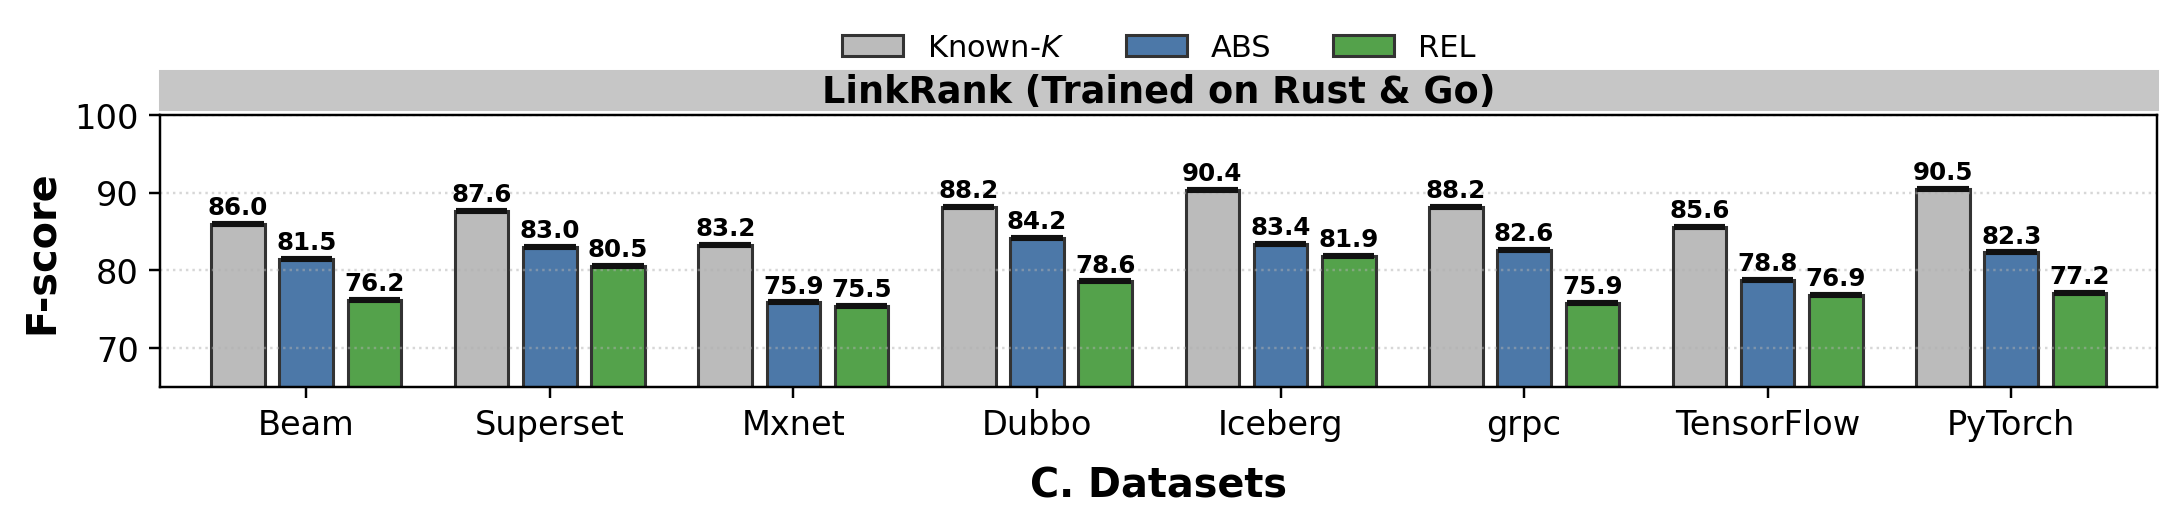
\includegraphics[width=\linewidth]{Figures/LR-rust.png}
  \caption{Cross-project performance of \textsc{LinkRank} trained on Go \& Rust repositories.}
  \label{fig:LR-rust}
\end{figure}

\begin{figure}[H]
  \centering
  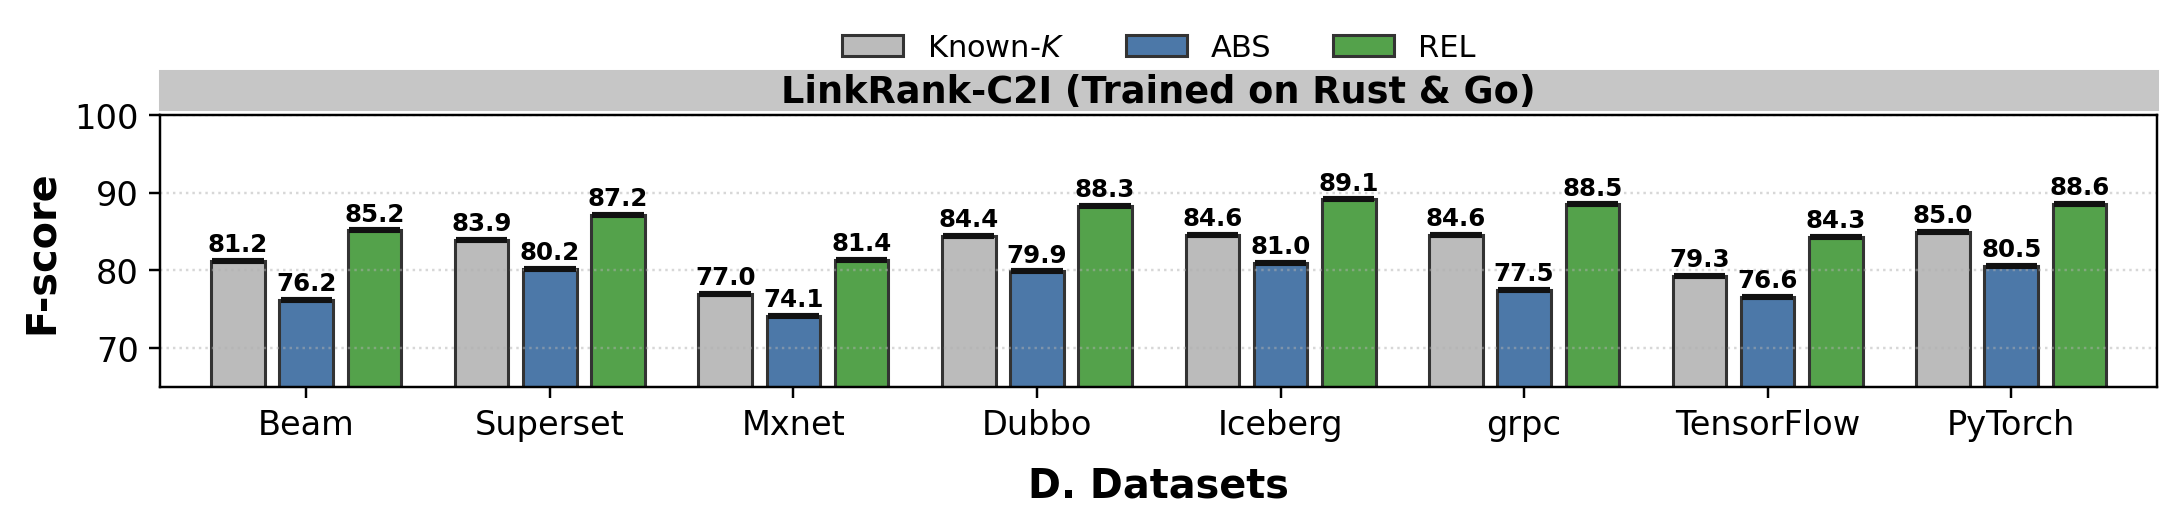
\includegraphics[width=\linewidth]{Figures/LR-C2I-rust.png}
  \caption{Cross-project performance of \textsc{LinkRank-C2I} trained on Go \& Rust repositories.}
  \label{fig:LR-C2I-rust}
\end{figure}


% =======================
%   TRAINED ON C++
% =======================
\begin{figure}[H]
  \centering
  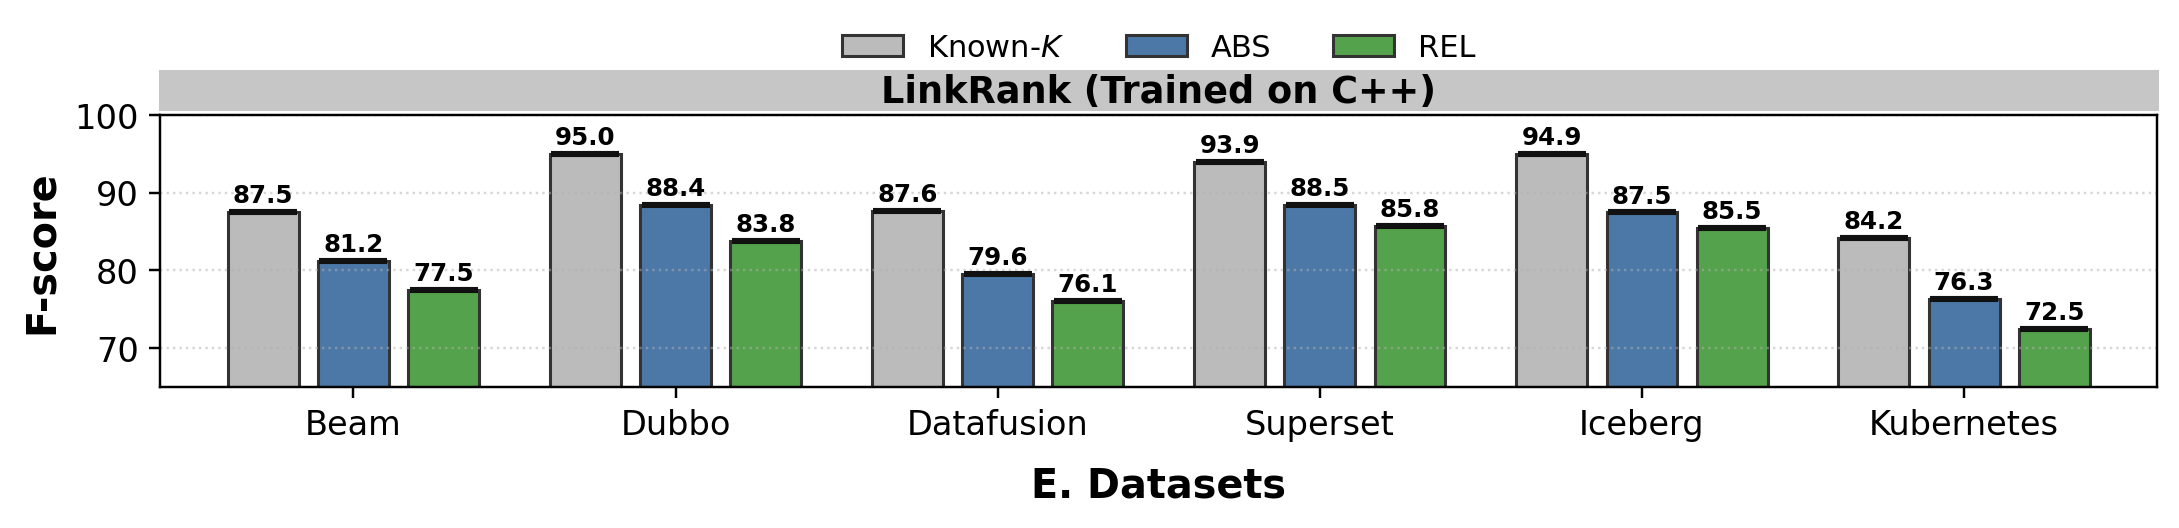
\includegraphics[width=\linewidth]{Figures/LR-cpp.png}
  \caption{Cross-project performance of \textsc{LinkRank} trained on C++ repositories.}
  \label{fig:LR-cpp}
\end{figure}

\begin{figure}[H]
  \centering
  \includegraphics[width=\linewidth]{Figures/lr-C2I-cpp.png}
  \caption{Cross-project performance of \textsc{LinkRank-C2I} trained on C++ repositories.}
  \label{fig:LR-C2I-cpp}
\end{figure}

Figures~\ref{fig:LR-java}--\ref{fig:LR-C2I-cpp} illustrate the cross-repository performance of LinkRank and LinkRank-C2I when trained on Java, Go \& Rust, and C++ repositories, respectively. For our proposed approaches, we observe a moderate performance drop compared to the non-cross-project setting. But considering the challenges of domain shift across programming languages and repository conventions, the models maintain competitive performance.\\


For LinkRank, training on Rust and Go leads to an approximate 5\% decrease in the ABS setting and around 7\% in the REL setting, highlighting the sensitivity of the model to language differences. For LinkRank-C2I, the decline is more pronounced, with about a 10\% drop under the Known-$K$ scenario and roughly 6\% in the ABS setting.  Despite these decreases, both models continue to achieve competitive scores across repositories, showing that our learning-to-rank framework remains effective and robust even in challenging cross-project scenarios.


% =======================
%   BASELINE METHODS
% =======================
\begin{figure}[H]
  \centering
  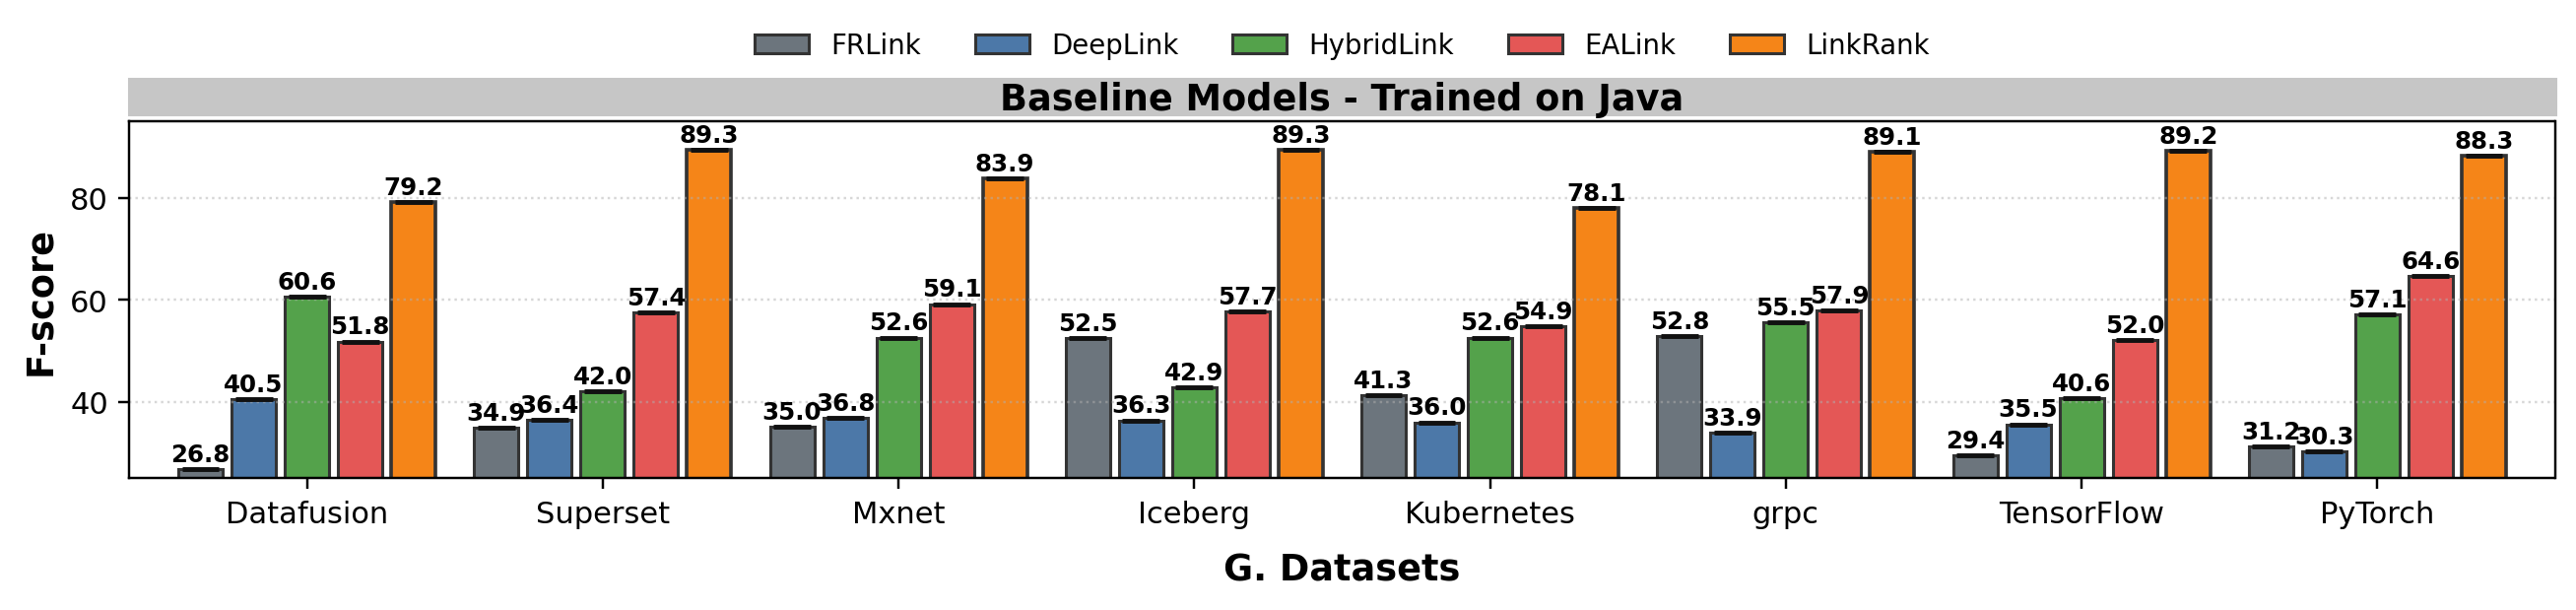
\includegraphics[width=\linewidth]{Figures/baseline_java.png}
  \caption{Baseline performance comparison for Java repositories}
  \subcaption*{(\textsc{FRLink}, \textsc{DeepLink}, \textsc{HybridLinker}, \textsc{EALink})}
  \label{fig:baseline_java}
\end{figure}

\begin{figure}[H]
  \centering
  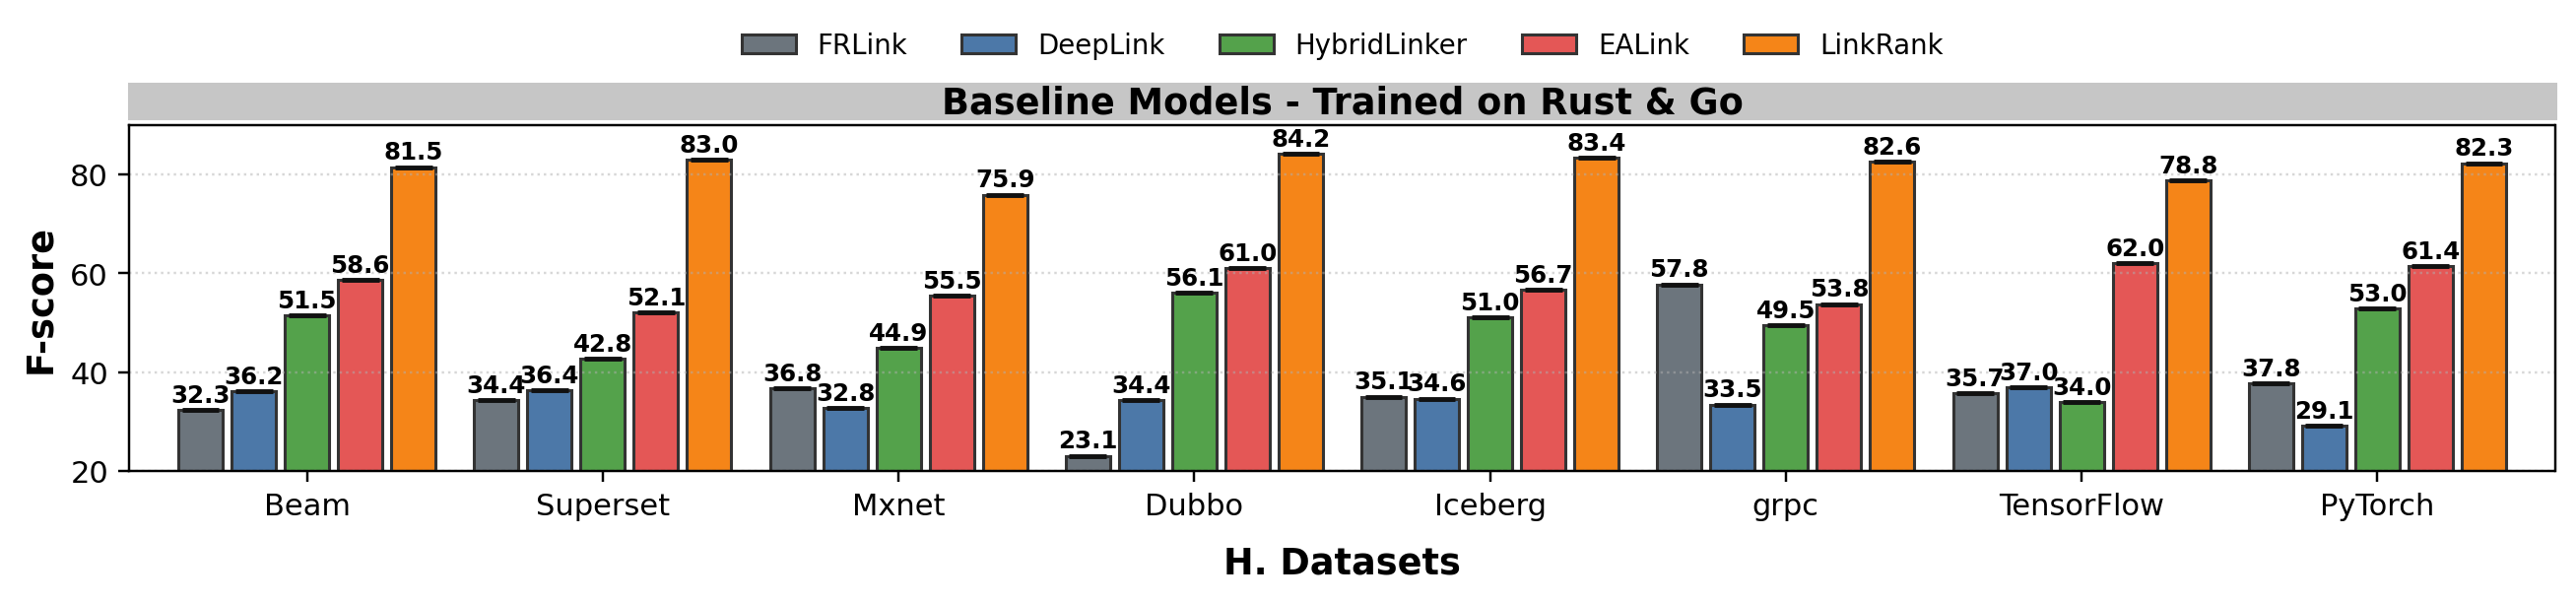
\includegraphics[width=\linewidth]{Figures/baseline_rust_go.png}
  \caption{Baseline performance comparison for Go \& Rust repositories.}
  \label{fig:baseline_rust_go}
\end{figure}

\begin{figure}[H]
  \centering
  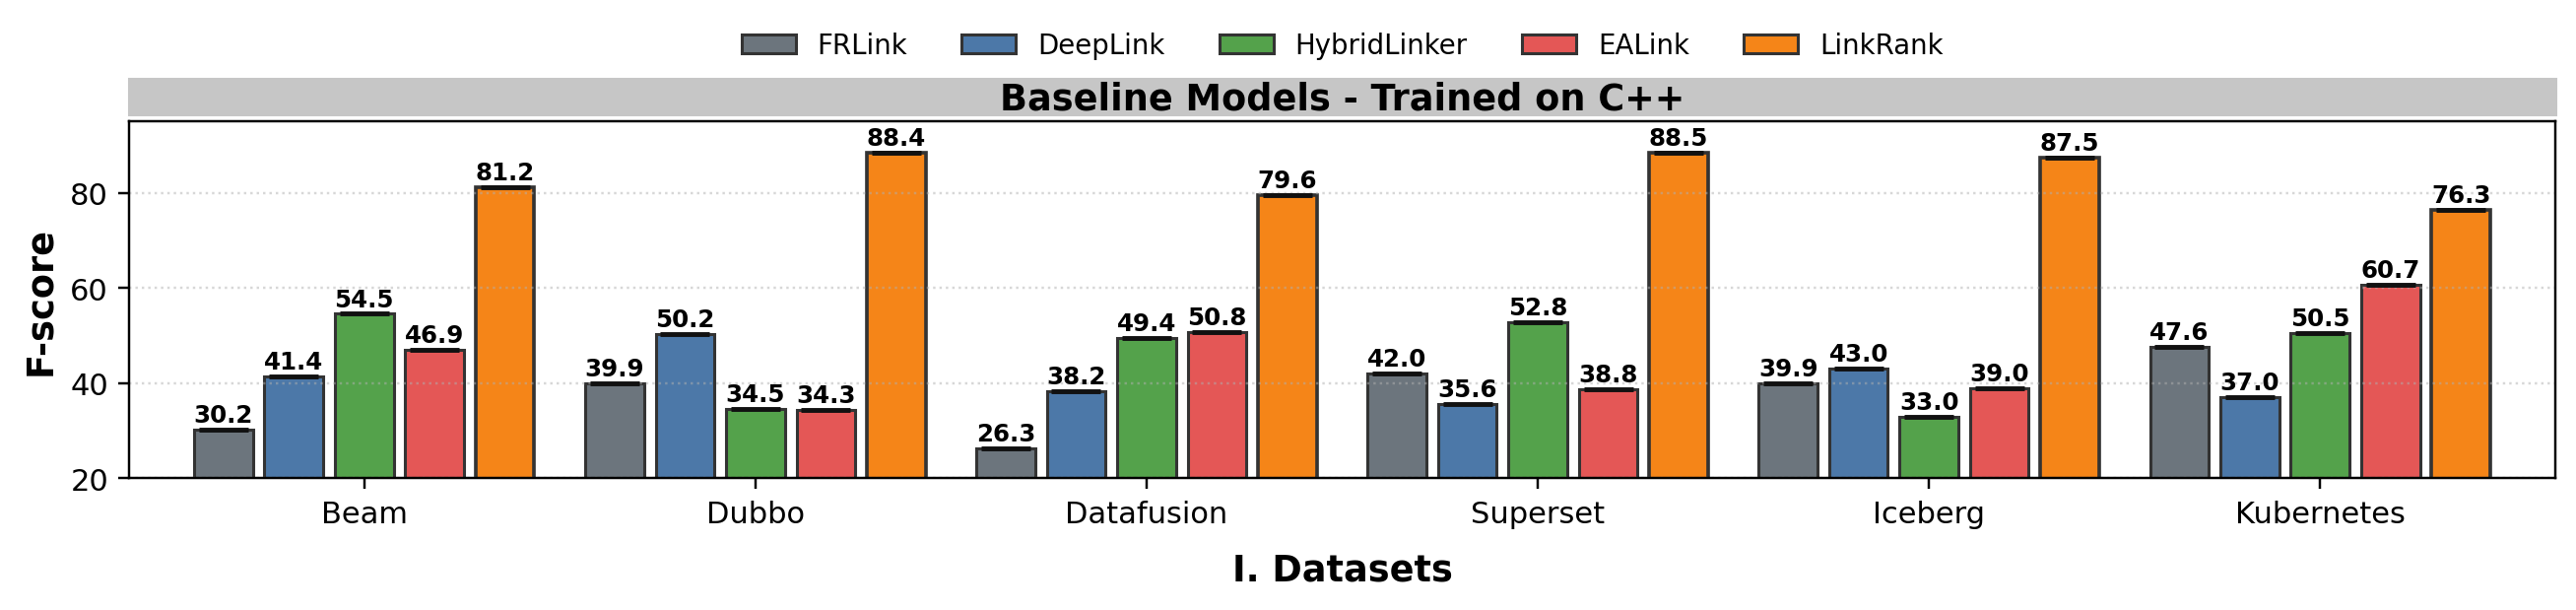
\includegraphics[width=\linewidth]{Figures/baseline_cpp.png}
  \caption{Baseline performance comparison for C++ repositories.}
  \label{fig:baseline_cpp}
\end{figure}

The baseline results can also be seen in the bar plots.  When we compute the average performance drop across all test datasets, FRLink shows the largest degradation, 19.24\% when trained on Rust and Go, and around 18\% when trained on either C++ or Java.  DeepLink drops by 14.27\% (Rust and Go), about 8\% (C++), and 13.51\% (Java).  HybridLinker exhibits 10.9\% (Rust and Go), 13.11\% (C++), and around 8\% (Java).  EALink is comparatively more stable, with about 4\% (Rust and Go), 16.4\% (C++), and 5.47\% (Java).  Taken together, the baselines experience non-trivial but heterogeneous losses under cross-project transfer, with EALink generally the most resilient and FRLink the most sensitive. Overall, we see that LinkRank remains comparatively more stable and effective across language boundaries than the baseline methods.